% !TeX root = RJwrapper.tex
\title{The \pkg{doBy} package for data handling, linear estimates and LS-means}
\author{by Søren Højsgaard}

\maketitle

\abstract{%
The \pkg{doBy} is one of several general utility packages on CRAN. We
illustrate two main features of the package: The ability to making
groupwise computations and the ability to compute linear estimates,
contrasts and least-squares means.
}

\hypertarget{introduction}{%
\subsection{Introduction}\label{introduction}}

The \CRANpkg{doBy} package \citep{doby} grew out of a need to calculate
groupwise summary statistics (much in the spirit of \code{PROC SUMMARY}
of the SAS system, \citep{procsummary}). The package first appeared on
CRAN, \url{https://cran-r-project.org}, in 2006. The name \pkg{doBy}
comes from the need to \textbf{do} some computations on data which is
stratified \textbf{By} the value of some variables. Today the package
contains many additional utilities. In this paper we focus 1) on the
``doing by''-functions and 2) on functions related to linear estimates
and contrasts (in particular LS-means).

\hypertarget{related-functionality}{%
\subsubsection{Related functionality}\label{related-functionality}}

When it comes to data handling, \pkg{doBy} is nowhere nearly as powerful
as more contemporary packages, such as those in the \CRANpkg{tidyverse}
eco system, \citep{tidyverse}. The \code{aggregate} function in base R
provides functionality similar to \pkg{doBy}s \code{summaryBy} function.
Another package to be mentioned in this connection is
\CRANpkg{data.table}, \citet{data.table}. On the other hand, \pkg{doBy}
is based on classical data structures that are unlikely to undergo
sudden changes. There is one exception to this, though: The data
handling functions work on tibble`s, from \CRANpkg{tibble}
\citet{tibble}. In relation to linear estimates, the \CRANpkg{multcomp}
package \citep{multcomp} deserves mention, and the \CRANpkg{lsmeans}
package \citep{lsmeans} provides facilities for computing LS-means.

It can be hypothesized that the data handling functions in \pkg{doBy}
remain appealing to a group of users because of their simplicity.

\hypertarget{functions-related-to-groupwise-computations}{%
\subsection{Functions related to groupwise
computations}\label{functions-related-to-groupwise-computations}}

\hypertarget{a-working-dataset---the-co2-data}{%
\subsubsection{\texorpdfstring{A working dataset - the \texttt{CO2}
data}{A working dataset - the CO2 data}}\label{a-working-dataset---the-co2-data}}

The \texttt{CO2} data frame comes from an experiment on the cold
tolerance of the grass species \emph{Echinochloa crus-galli}.
\texttt{Type} is a factor with levels \texttt{Quebec} or
\texttt{Mississippi} giving the origin of the plant. \texttt{Treatment}
is a factor levels \texttt{nonchilled} or \texttt{chilled}. Data is
balanced with respect to these two factors. However, illustrated certain
points we exclude a few rows of data to make data imbalanced. To limit
the amount of output we modify names and levels of variables as follows

\begin{Schunk}
\begin{Sinput}
data(CO2)
CO2 <- within(CO2, {
    Treat = Treatment; Treatment = NULL
    levels(Treat) = c("nchil", "chil"); levels(Type) = c("Que", "Mis")
})
CO2 <- subset(CO2, Plant %in% c("Qn1", "Qc1", "Mn1", "Mc1"))
CO2 <- CO2[-(1:3),]
xtabs(~Treat+Type, data=CO2)
\end{Sinput}
\begin{Soutput}
#>        Type
#> Treat   Que Mis
#>   nchil   4   7
#>   chil    7   7
\end{Soutput}
\begin{Sinput}
head(CO2, 4)
\end{Sinput}
\begin{Soutput}
#>   Plant Type conc uptake Treat
#> 4   Qn1  Que  350   37.2 nchil
#> 5   Qn1  Que  500   35.3 nchil
#> 6   Qn1  Que  675   39.2 nchil
#> 7   Qn1  Que 1000   39.7 nchil
\end{Soutput}
\end{Schunk}

\begin{Schunk}
\begin{figure}
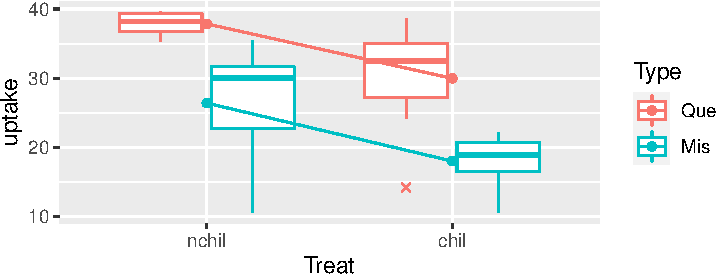
\includegraphics[keepaspectratio]{doby-hojsgaard-fig-interaction-1} \caption[Interaction plot for the CO2 data]{Interaction plot for the CO2 data. Boxplot outliers are crosses. The plot suggests additivity between Treat and Type.}\label{fig:interaction}
\end{figure}
\end{Schunk}

\hypertarget{the-function}{%
\subsubsection{\texorpdfstring{The \code{summaryBy}
function}{The  function}}\label{the-function}}

The \code{summaryBy} function is used for calculating quantities like
\emph{the mean and variance of numerical variables x and y for each
combination of two factors A and B}. Notice: A functionality similar to
\code{summaryBy} is provided by \code{aggregate} from base R, but
\code{summaryBy} offers additional features.

\begin{Schunk}
\begin{Sinput}
myfun1 <- function(x){c(m=mean(x), s=sd(x))}
summaryBy(cbind(conc, uptake, lu=log(uptake)) ~ Plant, data=CO2, FUN=myfun1)
\end{Sinput}
\begin{Soutput}
#>   Plant conc.m conc.s uptake.m uptake.s  lu.m    lu.s
#> 1   Qn1  631.2  279.4    37.85    2.014 3.633 0.05375
#> 2   Qc1  435.0  317.7    29.97    8.335 3.356 0.34457
#> 3   Mn1  435.0  317.7    26.40    8.694 3.209 0.42341
#> 4   Mc1  435.0  317.7    18.00    4.119 2.864 0.26219
\end{Soutput}
\end{Schunk}

The convention is that variables that do not appear in the dataframe
(e.g.~\code{log(uptake)}) must be named (here as \code{lu}). Various
shortcuts are available, e.g.~the following, where left hand side dot
refers to \emph{all numeric variables} while the right hand side dot
refers to \emph{all factor variables}. Writing \texttt{1} on the right
hand side leads to computing over the entire dataset:

\begin{Schunk}
\begin{Sinput}
summaryBy(. ~ ., data=CO2, FUN=myfun1)
\end{Sinput}
\begin{Soutput}
#>   Plant Type Treat conc.m conc.s uptake.m uptake.s
#> 1   Qn1  Que nchil  631.2  279.4    37.85    2.014
#> 2   Qc1  Que  chil  435.0  317.7    29.97    8.335
#> 3   Mn1  Mis nchil  435.0  317.7    26.40    8.694
#> 4   Mc1  Mis  chil  435.0  317.7    18.00    4.119
\end{Soutput}
\begin{Sinput}
summaryBy(. ~ 1, data=CO2, FUN=myfun1)
\end{Sinput}
\begin{Soutput}
#>   conc.m conc.s uptake.m uptake.s
#> 1  466.4  301.4    26.88    9.323
\end{Soutput}
\end{Schunk}

\hypertarget{specifications-as-formulas-and-lists}{%
\subsubsection{Specifications as formulas and
lists}\label{specifications-as-formulas-and-lists}}

The convention for the ``By''-functions is that a two sided formula like
can be written in two ways:

\begin{Schunk}
\begin{Sinput}
cbind(x, y) ~ A + B
list(c("x", "y"), c("A", "B"))
\end{Sinput}
\end{Schunk}

Some ``By''-functions only take a right hand sided formula as input.
Such a formula can also be written in two ways:

\begin{Schunk}
\begin{Sinput}
~ A + B
c("A", "B")
\end{Sinput}
\end{Schunk}

The list-form / vector-form is especially useful if a function is
invoked programatically. Hence the calls to \code{summaryBy} above can
also be made as

\begin{Schunk}
\begin{Sinput}
summaryBy(list(c("conc", "uptake", "lu=log(uptake)"), "Plant"), data=CO2, FUN=myfun1)
summaryBy(list(".", "."), data=CO2, FUN=myfun1)
summaryBy(list(".", "1"), data=CO2, FUN=myfun1)
\end{Sinput}
\end{Schunk}

\hypertarget{using-the-pipe-operator}{%
\subsection{Using the pipe operator}\label{using-the-pipe-operator}}

The \code{summaryBy} function has a counterpart called
\code{summary\_by}. The difference is that a formula is the first
argument to the former function while a dataframe (or a tibble) is the
first argument to the latter. The same applies to the other
``By''-functions. This allows for elegant use of the pipe operator
\texttt{\%\textgreater{}\%} from \CRANpkg{magrittr}, \citep{magrittr}:

\begin{Schunk}
\begin{Sinput}
CO2 %>% summary_by(cbind(conc, uptake) ~ Plant + Type, FUN=myfun1) -> newdat
newdat
\end{Sinput}
\begin{Soutput}
#>   Plant Type conc.m conc.s uptake.m uptake.s
#> 1   Qn1  Que  631.2  279.4    37.85    2.014
#> 2   Qc1  Que  435.0  317.7    29.97    8.335
#> 3   Mn1  Mis  435.0  317.7    26.40    8.694
#> 4   Mc1  Mis  435.0  317.7    18.00    4.119
\end{Soutput}
\end{Schunk}

\hypertarget{the-function-1}{%
\subsubsection{\texorpdfstring{The \code{orderBy}
function}{The  function}}\label{the-function-1}}

Ordering (or sorting) a data frame is possible with the \texttt{orderBy}
function. Suppose we want to order the rows of the the \texttt{CO2} data
by increasing values of \texttt{conc} and decreasing value of
\texttt{uptake} (within \texttt{conc}):

\begin{Schunk}
\begin{Sinput}
x1 <- orderBy(~ conc - uptake, data=CO2)
head(x1)
\end{Sinput}
\begin{Soutput}
#>    Plant Type conc uptake Treat
#> 22   Qc1  Que   95   14.2  chil
#> 43   Mn1  Mis   95   10.6 nchil
#> 64   Mc1  Mis   95   10.5  chil
#> 23   Qc1  Que  175   24.1  chil
#> 44   Mn1  Mis  175   19.2 nchil
#> 65   Mc1  Mis  175   14.9  chil
\end{Soutput}
\end{Schunk}

\hypertarget{the-function-2}{%
\subsubsection{\texorpdfstring{The \code{splitBy}
function}{The  function}}\label{the-function-2}}

Suppose we want to split \texttt{CO2} into a list of dataframes:

\begin{Schunk}
\begin{Sinput}
x1 <- splitBy(~ Plant + Type, data=CO2)
x1
\end{Sinput}
\begin{Soutput}
#>   listentry Plant Type
#> 1   Qn1|Que   Qn1  Que
#> 2   Qc1|Que   Qc1  Que
#> 3   Mn1|Mis   Mn1  Mis
#> 4   Mc1|Mis   Mc1  Mis
\end{Soutput}
\end{Schunk}

The result is a list (with a few additional attributes):

\begin{Schunk}
\begin{Sinput}
lapply(x1, head, 2)
\end{Sinput}
\begin{Soutput}
#> $`Qn1|Que`
#>   Plant Type conc uptake Treat
#> 4   Qn1  Que  350   37.2 nchil
#> 5   Qn1  Que  500   35.3 nchil
#> 
#> $`Qc1|Que`
#>    Plant Type conc uptake Treat
#> 22   Qc1  Que   95   14.2  chil
#> 23   Qc1  Que  175   24.1  chil
#> 
#> $`Mn1|Mis`
#>    Plant Type conc uptake Treat
#> 43   Mn1  Mis   95   10.6 nchil
#> 44   Mn1  Mis  175   19.2 nchil
#> 
#> $`Mc1|Mis`
#>    Plant Type conc uptake Treat
#> 64   Mc1  Mis   95   10.5  chil
#> 65   Mc1  Mis  175   14.9  chil
\end{Soutput}
\end{Schunk}

\hypertarget{the-function-3}{%
\subsubsection{\texorpdfstring{The \code{subsetBy}
function}{The  function}}\label{the-function-3}}

Suppose we want to select those rows within each treatment for which the
uptake is larger than 75\% quantile of uptake (within the treatment).
This is achieved by:

\begin{Schunk}
\begin{Sinput}
x2 <- subsetBy(~ Treat, subset=uptake > quantile(uptake, prob=0.75), data=CO2)
head(x2, 4)
\end{Sinput}
\begin{Soutput}
#>         Plant Type conc uptake Treat
#> nchil.4   Qn1  Que  350   37.2 nchil
#> nchil.6   Qn1  Que  675   39.2 nchil
#> nchil.7   Qn1  Que 1000   39.7 nchil
#> chil.25   Qc1  Que  350   34.6  chil
\end{Soutput}
\end{Schunk}

\hypertarget{the-function-4}{%
\subsubsection{\texorpdfstring{The \code{transformBy}
function}{The  function}}\label{the-function-4}}

The \code{transformBy} function is analogous to the \code{transform}
function except that it works within groups. For example:

\begin{Schunk}
\begin{Sinput}
x3 <- transformBy(~ Treat, data=CO2, 
                 minU=min(uptake), maxU=max(uptake), range=diff(range(uptake)))
head(x3, 4)
\end{Sinput}
\begin{Soutput}
#>   Plant Type conc uptake Treat minU maxU range
#> 1   Qn1  Que  350   37.2 nchil 10.6 39.7  29.1
#> 2   Qn1  Que  500   35.3 nchil 10.6 39.7  29.1
#> 3   Qn1  Que  675   39.2 nchil 10.6 39.7  29.1
#> 4   Qn1  Que 1000   39.7 nchil 10.6 39.7  29.1
\end{Soutput}
\end{Schunk}

\hypertarget{the-function-5}{%
\subsubsection{\texorpdfstring{The \code{lmBy}
function}{The  function}}\label{the-function-5}}

The \code{lmBy} function allows for fitting linear models to different
strata of data (the vertical bar is used for defining groupings of
data):

\begin{Schunk}
\begin{Sinput}
m <- lmBy(uptake ~ conc | Treat, data=CO2)
coef(m)
\end{Sinput}
\begin{Soutput}
#>       (Intercept)    conc
#> nchil       19.32 0.02221
#> chil        17.02 0.01602
\end{Soutput}
\end{Schunk}

The result is a list with a few additional attributes and the list can
be processed further as e.g.

\begin{Schunk}
\begin{Sinput}
lapply(m, function(z) coef(summary(z)))
\end{Sinput}
\begin{Soutput}
#> $nchil
#>             Estimate Std. Error t value  Pr(>|t|)
#> (Intercept) 19.31969   3.692936   5.232 0.0005408
#> conc         0.02221   0.006318   3.515 0.0065698
#> 
#> $chil
#>             Estimate Std. Error t value  Pr(>|t|)
#> (Intercept) 17.01814   3.668315   4.639 0.0005709
#> conc         0.01602   0.006986   2.293 0.0407168
\end{Soutput}
\end{Schunk}

\hypertarget{functions-related-linear-estimates-and-contrasts}{%
\subsection{Functions related linear estimates and
contrasts}\label{functions-related-linear-estimates-and-contrasts}}

A linear function of a \(p\)--dimensional parameter vector \(\beta\) has
the form \begin{displaymath}
  C=L\beta
\end{displaymath} where \(L\) is a \(q\times p\) matrix which we call
the \emph{Linear Estimate Matrix} or simply \emph{LE-matrix}. The
corresponding linear estimate is \(\hat C = L \hat \beta\). A linear
hypothesis has the form \(H_0: L\beta=m\) for some \(q\) dimensional
vector \(m\). In the following we describe what is essentially simple
ways of generating such \(L\)-matrices.

XXX: TEXT HERE

\begin{Schunk}
\begin{Sinput}
co2.add <- lm(uptake ~ Treat + Type, data=CO2)
co2.int <- lm(uptake ~ Treat * Type, data=CO2)
\end{Sinput}
\end{Schunk}

\hypertarget{computing-linear-estimates}{%
\subsubsection{Computing linear
estimates}\label{computing-linear-estimates}}

For now, we focus on the additive model. Consider computing the
estimated uptake for each treatment for plants originating from
Mississippi: One option: Construct the LE--matrix \(L\) directly and
then compute \(L\hat\beta\) as \texttt{L\ \%*\%\ coef(co2.add)}:

\begin{Schunk}
\begin{Sinput}
L <- matrix(c(1, 0, 1, 
              1, 1, 1), nrow=2, byrow=T)
L
\end{Sinput}
\begin{Soutput}
#>      [,1] [,2] [,3]
#> [1,]    1    0    1
#> [2,]    1    1    1
\end{Soutput}
\begin{Sinput}
L %*% coef(co2.add)
\end{Sinput}
\begin{Soutput}
#>       [,1]
#> [1,] 26.29
#> [2,] 18.11
\end{Soutput}
\end{Schunk}

In \pkg{doBy} there are facilities for computing \(L\) automatically and
for supplying \(L\hat\beta\) with standard errors etc.

\begin{Schunk}
\begin{Sinput}
L <- LE_matrix(co2.add, effect = "Treat", at=list(Type="Mis"))
L
\end{Sinput}
\begin{Soutput}
#>      (Intercept) Treatchil TypeMis
#> [1,]           1         0       1
#> [2,]           1         1       1
\end{Soutput}
\end{Schunk}

\begin{Schunk}
\begin{Sinput}
c1 <- linest(co2.add, L)
coef(c1)
\end{Sinput}
\begin{Soutput}
#>   estimate std.error statistic df   p.value
#> 1    26.29     2.247     11.70 22 6.440e-11
#> 2    18.11     2.247      8.06 22 5.209e-08
\end{Soutput}
\begin{Sinput}
confint(c1)
\end{Sinput}
\begin{Soutput}
#>   0.025 0.975
#> 1 21.63 30.95
#> 2 13.45 22.77
\end{Soutput}
\end{Schunk}

The function \code{esticon} has been part of \pkg{doBy} for many years
while \code{linest} is a newer addition. The functionality, however, is
similar:

\begin{Schunk}
\begin{Sinput}
c1 <- esticon(co2.add, L)
c1
\end{Sinput}
\begin{Soutput}
#>      estimate std.error statistic  p.value    beta0 df
#> [1,] 2.63e+01  2.25e+00  1.17e+01 6.44e-11 0.00e+00 22
#> [2,] 1.81e+01  2.25e+00  8.06e+00 5.21e-08 0.00e+00 22
\end{Soutput}
\end{Schunk}

\hypertarget{least-squares-means-lsmeans}{%
\subsubsection{Least-squares means
(LS--means)}\label{least-squares-means-lsmeans}}

A related question is: What is the estimated uptake for each treatment
if we ignore the type (i.e.~origin of the plants)? One option would to
fit a linear model without \texttt{Type} as explanatory variable:

\begin{Schunk}
\begin{Sinput}
co2.0 <- update(co2.add, . ~ . - Type)
L0 <- LE_matrix(co2.0, effect="Treat")
L0
\end{Sinput}
\begin{Soutput}
#>      (Intercept) Treatchil
#> [1,]           1         0
#> [2,]           1         1
\end{Soutput}
\begin{Sinput}
linest(co2.0, L=L0)
\end{Sinput}
\begin{Soutput}
#> Coefficients:
#>      estimate std.error statistic    df p.value
#> [1,]    30.56      2.68     11.40 23.00       0
#> [2,]    23.99      2.38     10.09 23.00       0
\end{Soutput}
\end{Schunk}

An alternative would be to stick to the original model but compute the
estimated uptake for each treatment for an \emph{average location}. That
would correspond to giving weight \(1/2\) to each of the two locations.
However, as one of the parameters is already set to zero to obtain
identifiability, we obtain the LE--matrix \(L\) as

\begin{Schunk}
\begin{Sinput}
L1 <- matrix(c(1, 0, 0.5, 
               1, 1, 0.5), nrow=2, byrow=T)
L1
\end{Sinput}
\begin{Soutput}
#>      [,1] [,2] [,3]
#> [1,]    1    0  0.5
#> [2,]    1    1  0.5
\end{Soutput}
\begin{Sinput}
linest(co2.add, L=L1)
\end{Sinput}
\begin{Soutput}
#> Coefficients:
#>      estimate std.error statistic    df p.value
#> [1,]    32.17      2.05     15.68 22.00       0
#> [2,]    23.99      1.79     13.41 22.00       0
\end{Soutput}
\end{Schunk}

Such a particular linear estimate is sometimes called a
\emph{least-squares mean}, an \emph{LSmean}, a \emph{marginal mean} or a
\emph{population mean}. Notice: One may generate \(L\) automatically
with

\begin{Schunk}
\begin{Sinput}
L1 <- LE_matrix(co2.add, effect="Treat")
L1
\end{Sinput}
\begin{Soutput}
#>      (Intercept) Treatchil TypeMis
#> [1,]           1         0     0.5
#> [2,]           1         1     0.5
\end{Soutput}
\end{Schunk}

Notice: One may obtain the LSmean directly as:

\begin{Schunk}
\begin{Sinput}
LSmeans(co2.add, effect="Treat")
## same as
linest(co2.add, L=LE_matrix(co2.add, effect="Treat"))
\end{Sinput}
\end{Schunk}

For a model with interactions, the LSmeans are computed as above, but
the \(L\)-matrix is:

\begin{Schunk}
\begin{Sinput}
LE_matrix(co2.int, effect="Treat")
\end{Sinput}
\begin{Soutput}
#>      (Intercept) Treatchil TypeMis Treatchil:TypeMis
#> [1,]           1         0     0.5               0.0
#> [2,]           1         1     0.5               0.5
\end{Soutput}
\end{Schunk}

\hypertarget{using-transformed-covariates}{%
\subsubsection{Using (transformed)
covariates}\label{using-transformed-covariates}}

Covariates are fixed at their average value (unless the
\texttt{at=...}-argument is used, see below). For example, \texttt{conc}
is fixed at the average value:

\begin{Schunk}
\begin{Sinput}
co2.lm1 <- lm(uptake ~ conc + Type + Treat, data=CO2)
lsm1 <- LSmeans(co2.lm1, effect="Treat")
lsm1
\end{Sinput}
\begin{Soutput}
#> Coefficients:
#>      estimate std.error statistic    df p.value
#> [1,]    31.33      1.39     22.58 21.00       0
#> [2,]    24.50      1.21     20.32 21.00       0
\end{Soutput}
\begin{Sinput}
lsm1$L
\end{Sinput}
\begin{Soutput}
#>      (Intercept)  conc TypeMis Treatchil
#> [1,]           1 466.4     0.5         0
#> [2,]           1 466.4     0.5         1
\end{Soutput}
\begin{Sinput}
lsm1a <- LSmeans(co2.lm1, effect="Treat", at=list(conc=700))
lsm1a
\end{Sinput}
\begin{Soutput}
#> Coefficients:
#>      estimate std.error statistic    df p.value
#> [1,]    35.14      1.49     23.59 21.00       0
#> [2,]    28.31      1.46     19.45 21.00       0
\end{Soutput}
\begin{Sinput}
lsm1a$L
\end{Sinput}
\begin{Soutput}
#>      (Intercept) conc TypeMis Treatchil
#> [1,]           1  700     0.5         0
#> [2,]           1  700     0.5         1
\end{Soutput}
\end{Schunk}

A special issue arises in connection with transformed covariates.
Consider:

\begin{Schunk}
\begin{Sinput}
co2.lm2 <- lm(uptake ~ conc + I(conc^2) + log(conc) + Type + Treat, data=CO2)
lsm2 <- LSmeans(co2.lm2, effect="Treat")
lsm2
\end{Sinput}
\begin{Soutput}
#> Coefficients:
#>      estimate std.error statistic     df p.value
#> [1,]   33.837     0.988    34.238 19.000       0
#> [2,]   27.472     0.964    28.488 19.000       0
\end{Soutput}
\begin{Sinput}
lsm2$L
\end{Sinput}
\begin{Soutput}
#>      (Intercept)  conc I(conc^2) log(conc) TypeMis Treatchil
#> [1,]           1 466.4    217529     6.145     0.5         0
#> [2,]           1 466.4    217529     6.145     0.5         1
\end{Soutput}
\end{Schunk}

Above \verb'I(conc^2)' is the the square of the average of \texttt{conc}
(which is \ensuremath{2.1753\times 10^{5}}) - not the average of the
squared values of \texttt{conc} (which is
\ensuremath{3.0476\times 10^{5}}). Likewise \texttt{log(conc)} is the
log of the average of \texttt{conc} (which is 6.145) - not the average
of the log of \texttt{conc} (which is 5.908). To make computations based
on the average value of the square of \texttt{conc} and the average of
the log of \texttt{conc} do

\begin{Schunk}
\begin{Sinput}
co2.lm3 <- lm(uptake ~ conc + conc2 + log.conc + Type + Treat, 
              data=transform(CO2, conc2=conc^2, log.conc=log(conc)))
lsm3 <- LSmeans(co2.lm3, effect="Treat")
lsm3
\end{Sinput}
\begin{Soutput}
#> Coefficients:
#>      estimate std.error statistic     df p.value
#> [1,]   31.041     0.838    37.019 19.000       0
#> [2,]   24.676     0.727    33.923 19.000       0
\end{Soutput}
\begin{Sinput}
lsm3$L
\end{Sinput}
\begin{Soutput}
#>      (Intercept)  conc  conc2 log.conc TypeMis Treatchil
#> [1,]           1 466.4 304758    5.908     0.5         0
#> [2,]           1 466.4 304758    5.908     0.5         1
\end{Soutput}
\end{Schunk}

If we want to evaluate the LS--means at \texttt{conc=700} then we can
do:

\begin{Schunk}
\begin{Sinput}
lsm4 <- LSmeans(co2.lm3, effect="Treat", at=list(conc=700, conc2=700^2, log.conc=log(700)))
lsm4
\end{Sinput}
\begin{Soutput}
#> Coefficients:
#>      estimate std.error statistic    df p.value
#> [1,]    34.93      1.19     29.41 19.00       0
#> [2,]    28.57      1.22     23.33 19.00       0
\end{Soutput}
\begin{Sinput}
lsm4$L
\end{Sinput}
\begin{Soutput}
#>      (Intercept) conc  conc2 log.conc TypeMis Treatchil
#> [1,]           1  700 490000    6.551     0.5         0
#> [2,]           1  700 490000    6.551     0.5         1
\end{Soutput}
\end{Schunk}

\hypertarget{alternative-models}{%
\subsection{Alternative models}\label{alternative-models}}

The functions \texttt{esticon}, \texttt{linest}, \texttt{LSmeans} etc.
are available for a range of model classes. We illustrate a few below:
We may decide to treat \verb|supp| as a random effect. This leads to a
\emph{linear mixed effects model} as implemented in \CRANpkg{lme4},
\citep{lme4}:

\begin{Schunk}
\begin{Sinput}
library(lme4)
#tooth.mix <- lmer(len ~ dose + (1|supp), data=ToothGrowth)
#LSmeans(tooth.mix, effect="dose")
co2.mix <- lmer(uptake ~ Treat + (1|Type), data=CO2)
LSmeans(co2.mix, effect="Treat")
\end{Sinput}
\begin{Soutput}
#> Coefficients:
#>      estimate std.error statistic    df p.value
#> [1,]    32.08      6.08      5.28  1.14    0.10
#> [2,]    23.99      5.99      4.00  1.08    0.14
\end{Soutput}
\end{Schunk}

Notice here that the parameter estimates themselves are similar to those
of a linear model (had data been completely balanced, the estimates
would have been identical). However, the standard errors of the the
estimates are much larger under the mixed model. This is due to
\texttt{supp} being treated as a random effect. Notice that the degrees
of freedom by default are adjusted using a Kenward--Roger approximation
(provided that \CRANpkg{pbkrtest} package \citep{pbkrtest} is
installed). Adjustment of degrees of freedom is controlled with the
\texttt{adjust.df} argument. LS-means are also available in a
\emph{generalized linear model} setting as well as for for
\emph{generalized estimating equations} as implemented in the
\CRANpkg{geepack} package, \citep{geepack}. In both cases the LS--means
are on the scale of the linear predictor - not on the scale of the
response. For example:

\begin{Schunk}
\begin{Sinput}
co2.glm <- glm(uptake ~ Treat + Type, family=Gamma("identity"), data=CO2)
LSmeans(co2.glm, effect="Treat")
\end{Sinput}
\begin{Soutput}
#> Coefficients:
#>      estimate std.error statistic p.value
#> [1,]    32.23      2.41     13.40       0
#> [2,]    23.95      1.64     14.62       0
\end{Soutput}
\begin{Sinput}
library(geepack)
co2.gee <- geeglm(uptake ~ Treat, id=Type, family=Gamma("identity"), data=CO2)
LSmeans(co2.gee, effect="Treat")
\end{Sinput}
\begin{Soutput}
#> Coefficients:
#>      estimate std.error statistic p.value
#> [1,]    30.56      3.75      8.16       0
#> [2,]    23.99      4.23      5.67       0
\end{Soutput}
\end{Schunk}

\hypertarget{acknowledgements}{%
\subsection{Acknowledgements}\label{acknowledgements}}

Credit is due to Dennis Chabot, Gabor Grothendieck, Paul Murrell, Jim
Robison-Cox and Erik Jørgensen for reporting various bugs and making
various suggestions to the functionality in the \pkg{doBy} package.

\bibliography{doby-hojsgaard}


\address{%
Søren Højsgaard\\
Department of Mathematical Sciences, Aalborg University, Denmark\\
Skjernvej 4A\\ 9220 Aalborg Ø, Denmark\\
}
\href{mailto:sorenh@math.aau.dk}{\nolinkurl{sorenh@math.aau.dk}}

